\documentclass[10pt]{article}
\usepackage[margin=1in]{geometry}
\usepackage{amsmath,amssymb}
\usepackage{graphicx}
\usepackage{booktabs}
\usepackage{natbib}
\usepackage{hyperref}
\usepackage{textcomp}

\title{An Artificial Intelligence Accelerated Virtual Screening Platform for Drug Discovery}
\author{[Authors]}
\date{}

\begin{document}
\maketitle

% ============================================================
% ABSTRACT
% ============================================================
\begin{abstract}
Structure-based virtual screening is central to early-stage drug discovery, yet
physics-based docking of multi-billion compound libraries remains constrained
by computational cost and scoring-function accuracy, while leading docking
programs are proprietary and open-source alternatives lack both flexible-receptor
modeling and active-learning triage. We present RosettaGenFF-VS, a physics-based
force field that extends Rosetta GALigandDock with new atom types, torsional
potentials, and an entropy model for ranking ligands against a common target.
We expose two docking modes---virtual screening express (VSX) for rapid library
triage and virtual screening high-precision (VSH) with full receptor sidechain
flexibility---and integrate them into OpenVS, an open-source AI-accelerated
virtual screening platform that trains a target-specific surrogate neural network
on-the-fly to select promising compounds for expensive docking. On CASF-2016,
RosettaGenFF-VS achieves a top~1\% enrichment factor of 16.72 versus 11.9 for
the second-best method; on the Directory of Useful Decoys, RosettaVS outperforms
the second-best method by a factor of two at 0.5/1.0\% ROC enrichment. Screening
approximately 5.5 billion Enamine REAL compounds against the KLHDC2 ubiquitin
ligase and approximately 4.1 billion ZINC22 compounds against NaV1.7 VSD4 each
completed in under seven days on a 3000-CPU / 1 RTX2080 GPU cluster, yielding
seven novel KLHDC2 binders (14\% hit rate, best IC$_{50} \sim 3$~\textmu M) and
four novel NaV1.7 antagonists (44.4\% hit rate, best inactivated-state
IC$_{50}$ = 1.32~\textmu M). A 2.0~\AA\ X-ray co-crystal structure of KLHDC2
with compound~29 validates the predicted binding pose.
\end{abstract}

% ============================================================
% INTRODUCTION (from intro_relwork.tex)
% ============================================================
\section{Introduction}

Structure-based virtual screening has become a central tool in small-molecule
lead discovery, offering a route to interrogate chemical space at a scale that
is impractical with wet-lab assays alone. The explosion of make-on-demand
ultra-large libraries, which now span billions of purchasable molecules with
high reported synthesis success rates, has dramatically expanded the pool of
candidate ligands that can in principle be evaluated against a target
\citep{lyu2019ultralarge,tingle2023zinc22,irwin2005zinc}. Yet only a handful of
virtual screening campaigns deployed at this multi-billion scale have
translated into experimentally validated hits, in part because exhaustive
physics-based docking of entire libraries is computationally prohibitive
\citep{gorgulla2020virtualflow,gentile2022deepdocking}.

Several strategies have emerged to address this cost. Parallelized docking
platforms distribute calculations across high-performance computing clusters
\citep{gorgulla2020virtualflow,yaacoub2022ddgui}; active-learning and
Bayesian-optimization approaches train surrogate models to triage libraries so
that only the most promising fraction must be docked
\citep{graff2021accelerating,gentile2022deepdocking}; hierarchical pipelines
apply successively more expensive scoring stages to progressively smaller
compound pools; and GPU-accelerated docking programs further compress
wall-clock time. However, the ultimate impact of any of these strategies is
bounded by the accuracy of the underlying docking program, which must both
sample a biologically meaningful binding pose and score it in a way that
distinguishes true binders from decoys.

Leading proprietary docking programs such as Glide \citep{friesner2004glide}
and the grey-wolf-optimized variants integrated into VirtualFlow
\citep{gorgulla2020virtualflowgwo} offer strong benchmarked performance but
are not freely available for unrestricted academic use. AutoDock Vina
\citep{trott2010vina} is free and widely adopted but tends to trail
commercial programs on standard benchmarks. Recent deep-learning scoring
functions report competitive numbers on benchmarks such as CASF-2016
\citep{su2019casf2016,liu2017pdbbind,scantlebury2023pointvs}, yet their ability
to generalize to novel compounds and targets is limited, and data-leakage
between training and evaluation sets remains a concern even when stringent
similarity cutoffs are applied. When the binding site is known, as is typical
in virtual screening, physics-based methods continue to be the pragmatic
choice \citep{chaput2017usc,ebejer2019ligity,li2024cache}. Open-source physics
based platforms that combine accurate force fields, receptor flexibility, and
active-learning triage for billion-compound libraries remain scarce.

In this work, we introduce RosettaGenFF-VS and the RosettaVS protocol, built
on top of the Rosetta GALigandDock framework \citep{leman2020rosetta}. We
extend the underlying generalized force field with new atom types, new
torsional potentials, and an entropy model so that it can rank large pools of
compounds binding to the same target. We expose two docking modes: a fast
virtual screening express (VSX) mode for initial library triage and a virtual
screening high-precision (VSH) mode that restores full receptor sidechain
flexibility for final re-ranking of top candidates. These are wrapped by
OpenVS, an open-source AI-accelerated virtual screening platform that trains
a target-specific surrogate model on-the-fly to select promising compounds
for expensive docking, enabling routine screens of multi-billion compound
libraries on modest HPC resources. We benchmark the method on CASF-2016
\citep{su2019casf2016} and the Directory of Useful Decoys
\citep{mysinger2012dude}, then apply the platform to two unrelated
drug-discovery problems: a substrate receptor in the CUL2/CRL2 ubiquitin
ligase family, KLHDC2, which has recently attracted attention as a PROTAC
platform \citep{slusarz2023klhdc3}, and the voltage-sensing domain IV (VSD4)
of the human voltage-gated sodium channel NaV1.7, a validated but notoriously
difficult target for state-dependent small-molecule inhibitors
\citep{wang2015nav17methyl}. The KLHDC2 co-crystal structure determined for
the best initial hit validates the predicted binding pose, and the NaV1.7
leads display state-dependent inhibition with moderate selectivity over
NaV1.5 and hERG.

The contributions of this work are:
\begin{itemize}
  \item \textbf{Force field}: RosettaGenFF-VS extends Rosetta GALigandDock
  \citep{leman2020rosetta} with new atom types, torsional potentials, and an
  entropy term for ranking ligands binding to the same target.
  \item \textbf{Protocol}: RosettaVS supplies paired VSX (fast) and VSH
  (flexible-receptor, high-precision) docking modes for ultra-large screens.
  \item \textbf{Platform}: OpenVS is an open-source scalable virtual
  screening platform that combines these modes with active-learning triage,
  enabling multi-billion compound screens in under seven days on modest HPC
  resources.
  \item \textbf{Benchmarks}: We report leading CASF-2016 docking and
  screening power (top 1\% enrichment factor of 16.72 versus 11.9 for the
  second-best method) and DUD ROC enrichment, outperforming the second-best
  method by a factor of two at 0.5/1.0\% false-positive rates.
  \item \textbf{Applications}: Parallel KLHDC2 and NaV1.7 campaigns yielded
  seven low-micromolar KLHDC2 binders (14\% hit rate) and four
  single-digit-micromolar NaV1.7 antagonists (44.4\% hit rate), the best of
  which showed state-dependent hNaV1.7 inhibition with IC$_{50}$ = 1.32~\textmu M.
  \item \textbf{Structural validation}: A 2.0~\AA\ X-ray co-crystal structure
  of KLHDC2 with compound~29 validates the predicted binding pose of the
  computationally identified hit.
\end{itemize}

% ============================================================
% BACKGROUND AND RELATED WORK (from intro_relwork.tex)
% ============================================================
\section{Background and Related Work}

\paragraph{Ultra-large library docking.}
Make-on-demand libraries have expanded chemical space from the millions to
the billions of compounds \citep{lyu2019ultralarge,tingle2023zinc22}. Early
examples of ultra-large screens demonstrated that hit rates and chemotype
diversity can improve with increasing library size
\citep{lyu2019ultralarge,gorgulla2020virtualflow}, motivating the development
of platforms that can evaluate billions of molecules efficiently.
VirtualFlow demonstrates distributed ultra-large screening against targets
such as KEAP1 \citep{gorgulla2020virtualflow}, and later extensions
incorporate receptor flexibility via grey-wolf optimization
\citep{gorgulla2020virtualflowgwo}.

\paragraph{Active learning and deep-learning-guided screening.}
Rather than docking an entire library, active-learning approaches train a
cheap surrogate on a small fraction of docked compounds and use it to triage
the rest. Pool-based Bayesian optimization can recover a large share of the
top-scoring ligands in a 100-million-compound library after docking only a
few percent of it \citep{graff2021accelerating}. Deep Docking and its
successors deploy iterative neural-network surrogates to accelerate ligand
ranking in conjunction with a conventional docker
\citep{gentile2022deepdocking,yaacoub2022ddgui}. Recent community exercises
such as CACHE suggest that while such acceleration is reliable, hit rates on
truly novel pockets remain modest, underscoring the importance of the
underlying scoring function \citep{li2024cache}.

\paragraph{Docking programs and scoring functions.}
Glide uses hierarchical conformational search with an empirical-plus-force-field
scoring function and reports strong redocking accuracy on standard
benchmarks \citep{friesner2004glide}. AutoDock Vina introduced a smoothed
empirical scoring function with efficient optimization and multithreading,
and remains a widely used open-source baseline \citep{trott2010vina}. The
PDBbind and CASF benchmarks quantify scoring, ranking, docking, and
screening power of scoring functions on diverse protein-ligand complexes
\citep{liu2017pdbbind,su2019casf2016}, while the Directory of Useful Decoys
and its enhanced version evaluate virtual-screening discrimination using
property-matched decoys \citep{mysinger2012dude}. Consensus docking analyses
and knowledge-based ligand methods illustrate both the strengths and the
failure modes of current approaches \citep{chaput2017usc,ebejer2019ligity}.

\paragraph{Machine-learning scoring functions.}
Neural-network scoring functions have shown competitive CASF numbers, yet
concerns about train/test leakage persist even when ligand Tanimoto and
protein sequence-identity cutoffs are applied. Recent work argues that
careful dataset construction and interpretability testing are needed before
these methods can be trusted as drop-in replacements for physics-based
scoring \citep{scantlebury2023pointvs}. Additionally, docking apo protein
structures typically degrades virtual-screening performance, motivating
flexible-receptor refinement and holo-like pocket conformation generation
\citep{guterres2020apo}.

\paragraph{KLHDC2 and NaV1.7 as test targets.}
KLHDC2 is a substrate receptor of the CUL2/CRL2 E3 ubiquitin ligase complex
and recognizes C-terminal diglycine degrons with high affinity
\citep{slusarz2023klhdc3}. Its tractable, pocket-like degron-binding site
has made it a candidate platform for PROTAC-style targeted protein
degradation. The human voltage-gated sodium channel NaV1.7, in turn, is a
well-validated analgesic target for which subtype-selective small-molecule
inhibitors have been pursued through interactions with the fourth
voltage-sensing domain (VSD4); subtle chemical modifications of known aryl
sulfonamide scaffolds can introduce new modes of gating modulation, making
the domain a rewarding but structurally subtle pocket for virtual screening
\citep{wang2015nav17methyl}. We chose these two targets to test the
generality of RosettaVS across protein folds, pocket physicochemistry, and
assay modalities.

\paragraph{This work.}
Against this backdrop, RosettaGenFF-VS, RosettaVS, and OpenVS combine an
open-source, physics-based scoring function with flexible-receptor docking
and active-learning triage. Unlike deep-learning scoring functions, the
method does not rely on the distribution of training ligands; unlike
proprietary commercial pipelines, all components are free and open-source;
and unlike previous active-learning approaches, receptor flexibility is
modeled at the final VSH stage. The benchmark and experimental results that
follow justify each of these choices.


% ============================================================
% METHODS
% ============================================================
\section{Methods}

\subsection{RosettaGenFF-VS Force Field}

RosettaGenFF-VS extends the Rosetta GALigandDock generalized force field
\citep{leman2020rosetta} for large-scale virtual screening applications.
Three principal modifications were introduced. First, the set of atom types
was expanded and new torsional potentials were added to improve the modeling
of functional groups encountered in multi-billion compound libraries that
were underrepresented in the original parameterization. Second, the
preprocessing pipeline was revised to improve robustness when handling the
diversity of input structures generated by cheminformatics toolkits at the
billion-compound scale. Third, an entropy model estimating the change in
configurational entropy upon ligand binding ($\Delta S$) was developed and
combined with the existing enthalpy model ($\Delta H$), yielding a free-energy
estimate ($\Delta G = \Delta H - T \Delta S$) suitable for ranking
structurally distinct ligands binding to the same target pocket.

\subsection{RosettaVS Docking Protocol}

RosettaVS implements two docking modes within Rosetta GALigandDock:

\begin{itemize}
  \item \textbf{Virtual Screening Express (VSX)}: a fast docking mode designed
  for rapid initial screening of multi-billion compound libraries. VSX employs
  a streamlined conformational search with the RosettaGenFF-VS scoring
  function but holds receptor sidechains fixed to reduce computational cost.
  \item \textbf{Virtual Screening High-precision (VSH)}: a more accurate
  docking mode used for final re-ranking of top hits from the initial VSX
  screen. VSH restores full receptor sidechain flexibility during docking,
  enabling the modeling of induced conformational changes upon ligand binding.
  This proves important for targets where pocket sidechains rearrange to
  accommodate structurally diverse ligands.
\end{itemize}

\subsection{OpenVS Platform}

The OpenVS platform integrates RosettaVS with active-learning triage to enable
routine screening of multi-billion compound libraries on modest HPC resources.
During docking, a target-specific surrogate neural network is trained
simultaneously on the accumulating docking scores. After each iteration, the
surrogate model selects the most promising subset of undocked compounds for
the next round of physics-based docking, so that only a small fraction
(approximately 0.11\% in the reported campaigns) of the full library is ever
explicitly docked. The platform was designed to be highly scalable and
parallelizable across thousands of CPUs.

\subsection{Benchmarks}

\paragraph{CASF-2016.}
The CASF-2016 dataset \citep{su2019casf2016} consists of 285 diverse
protein-ligand complexes drawn from PDBbind \citep{liu2017pdbbind}. Docking
power was assessed by the success rate of placing the top 1/2/3 predicted
poses within 2~\AA\ RMSD of the native structure. Screening power was
assessed by two metrics: (i) the enrichment factor at the top $X$\% cutoff
(EF$_{X\%}$), which measures early enrichment of true positives, and (ii) the
success rate of placing the best binder among the top 1\%/5\%/10\% ranked
ligands across all target proteins.

\paragraph{DUD.}
The Directory of Useful Decoys dataset \citep{mysinger2012dude} comprises
40 pharmaceutically relevant protein targets with over 100,000 small
molecules including both actives and property-matched decoys. Performance was
quantified by the area under the receiver operating characteristic curve (AUC)
and by ROC enrichment at 0.5\%, 1.0\%, and 2.0\% false-positive rates,
averaged over targets and over three independent runs.

\subsection{KLHDC2 Virtual Screening Campaign}

The Enamine REAL library (approximately 5.5 billion purchasable small molecules,
80\% synthesis success rate) was screened against KLHDC2 using the OpenVS
platform with VSX mode. Active learning was run for 10 iterations; the
predicted binding affinity of the top 0.1 percentile improved from
$-6.81$~kcal/mol (iteration~1) to $-12.43$~kcal/mol (iteration~10).
Approximately 6 million compounds (0.11\%) were subjected to docking. The
top 50,000 compounds were re-docked with VSH mode. The entire computation
completed within one week on a local HPC cluster equipped with 3000 CPUs and
one RTX2080 GPU.

The top 1,000 compounds from the VSH re-ranking were filtered for predicted
solubility and hydrogen-bond completeness, then similarity-clustered. A total
of 54 clustered candidates were examined manually; 37 were selected for
synthesis and 29 were successfully synthesized. Binding was assessed using an
AlphaLISA competition assay measuring displacement of a diglycine-containing
SelK C-end degron peptide from KLHDC2, with confirmation by BioLayer
Interferometry (BLI).

A focused follow-up screen searched ZINC22 \citep{tingle2023zinc22} for
compounds containing the acetyl-amino-methyl-triazole-acetic acid backbone
substructure, yielding approximately 381,567 hits. Twenty-one compounds were
synthesized and tested in the AlphaLISA assay.

X-ray crystallography was performed by soaking apo KLHDC2 crystals with
compound~29 (C29), and the structure of the KLHDC2--C29 complex was
determined at 2.0~\AA\ resolution.

\subsection{NaV1.7 VSD4 Virtual Screening Campaign}

The ZINC22 library \citep{tingle2023zinc22} (approximately 4.1 billion
compounds) was screened against the voltage-sensing domain IV (VSD4) of
hNaV1.7 using the same OpenVS/VSX pipeline. Active learning was run for
7 iterations; the predicted binding affinity of the top 0.1 percentile
improved from $-10.8$~kcal/mol (iteration~1) to $-18.2$~kcal/mol (final
iteration). Approximately 4.5 million compounds (0.11\%) were subjected to
docking. The top 100,000 were re-docked with VSH mode.

The top 100,000 compounds were clustered; the top 1,000 cluster
representatives were filtered; 160 molecules passing all filters were examined
manually. To ensure novelty, molecules containing known arylsulfonamide
warheads or structurally resembling antihistamines or beta-receptor blockers
were excluded. Ten molecules were selected (Tanimoto similarity $< 0.33$ to
known ChEMBL NaV1.7 inhibitors); 9 were successfully synthesized.

Activity was measured by whole-cell patch-clamp electrophysiology on hNaV1.7
stably expressed in HEK-293 cells. State-dependent inhibition was assessed by
comparing IC$_{50}$ values at inactivated-state ($-70$~mV holding potential)
and resting-state ($-120$~mV holding potential) conditions. Selectivity was
evaluated against hNaV1.5 and hERG channels.


% ============================================================
% RESULTS
% ============================================================
\section{Results}

% --- Pipeline schematic ---
\begin{figure}[htbp]
\centering

\includegraphics[width=0.85\textwidth]{figures/fig_pipeline.pdf}
\caption{Schematic overview of the OpenVS platform pipeline. An ultra-large
compound library (billions of molecules) is triaged by an active-learning
neural-network surrogate, docked with VSX (fast mode), re-ranked with VSH
(flexible-receptor mode), filtered and clustered, then advanced to synthesis
and experimental assay.}
\label{fig:pipeline}
\end{figure}

\subsection{Development of an AI-Accelerated Virtual Screening Platform}

RosettaGenFF-VS adds an entropy term ($\Delta S$) to the existing enthalpy
model in Rosetta GALigandDock \citep{leman2020rosetta}, yielding a composite
free-energy score for ranking structurally diverse ligands against a common
target. The expanded atom types and torsional potentials improve the
representation of functional groups encountered across multi-billion compound
libraries. The RosettaVS protocol exposes VSX and VSH docking modes, with
VSH incorporating full receptor sidechain flexibility for final re-ranking.
The OpenVS platform (Figure~\ref{fig:pipeline}) uses active-learning surrogate
training during docking to avoid evaluating the entire library, enabling
routine multi-billion compound screens on modest HPC resources.

\subsection{RosettaVS Achieves Leading Benchmark Performance}

\paragraph{CASF-2016 docking and screening power.}
On the CASF-2016 285-complex benchmark \citep{su2019casf2016}, RosettaGenFF-VS
achieves the leading success rate in placing the top 1/2/3 predicted poses
within 2~\AA\ RMSD of the native structure. In the screening power test, the
top~1\% enrichment factor from RosettaGenFF-VS
($\text{EF}_{1\%} = 16.72$) outperforms the second-best method
($\text{EF}_{1\%} = 11.9$) by a substantial margin
(Figure~\ref{fig:casf_ef1}). RosettaGenFF-VS also leads in the success rate of
identifying the best binder within the top 1\%/5\%/10\% ranked molecules.
Analysis on screening power subsets shows particular improvements on more
polar, shallower, and smaller protein pockets compared to other methods.

% --- CASF EF1% figure ---
\begin{figure}[htbp]
\centering
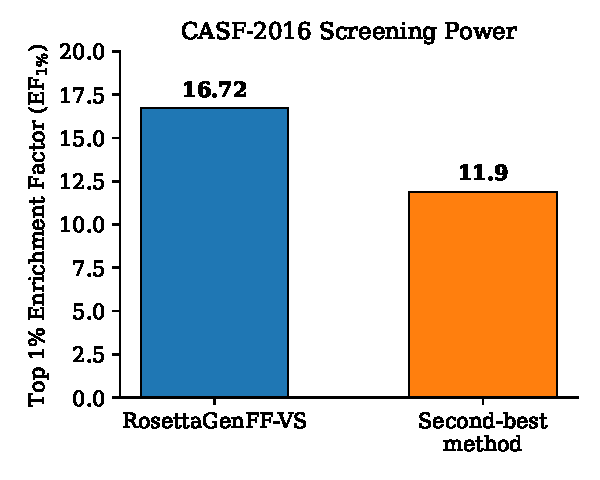
\includegraphics[width=0.55\textwidth]{figures/fig_casf_ef1.pdf}
\caption{CASF-2016 screening power comparison. Top 1\% enrichment factor
(EF$_{1\%}$) for RosettaGenFF-VS (16.72) versus the second-best method (11.9),
demonstrating a substantial margin in early-enrichment performance on the
285-complex benchmark.}
\label{fig:casf_ef1}
\end{figure}

% --- CASF screening power table ---
\begin{table}[htbp]
\centering
\caption{CASF-2016 screening power: top 1\% enrichment factor. RosettaGenFF-VS
versus the second-best method on the 285-complex benchmark.}
\label{tab:casf_screening}
\begin{tabular}{lc}
\toprule
Method & EF$_{1\%}$ \\
\midrule
RosettaGenFF-VS & 16.72 \\
Second-best method & 11.9 \\
\bottomrule
\end{tabular}
\end{table}

\paragraph{DUD virtual screening performance.}
On the DUD dataset \citep{mysinger2012dude} (40 targets, $>$100,000 molecules),
RosettaVS leads on both AUC and ROC enrichment metrics averaged over targets
and three independent runs. RosettaVS outperforms the second-best method by
a factor of two at 0.5\% and 1.0\% false-positive rates, representing a
substantial advance in early ROC enrichment. VSH mode slightly outperforms
VSX mode, attributable to the modeling of pocket sidechain conformational
changes induced by ligand binding.

\subsection{Discovery of Novel KLHDC2 Ubiquitin Ligase Binders}

The OpenVS platform screened the Enamine REAL library (approximately 5.5 billion
compounds, 80\% synthesis success rate) against KLHDC2 \citep{slusarz2023klhdc3}
using VSX mode. Over 10 active-learning iterations, the predicted binding
affinity of the top 0.1 percentile improved from $-6.81$~kcal/mol (iteration~1)
to $-12.43$~kcal/mol (iteration~10) (Figure~\ref{fig:active_learning}).
Screening was stopped after iteration~10, as no new global minimum structures
were identified beyond iteration~8. Approximately 6 million compounds (0.11\%)
were subjected to docking; the top 50,000 were re-docked with VSH mode. The
entire campaign completed within one week on a cluster with 3000 CPUs and
1 RTX2080 GPU.

% --- Active learning convergence figure ---
\begin{figure}[htbp]
\centering
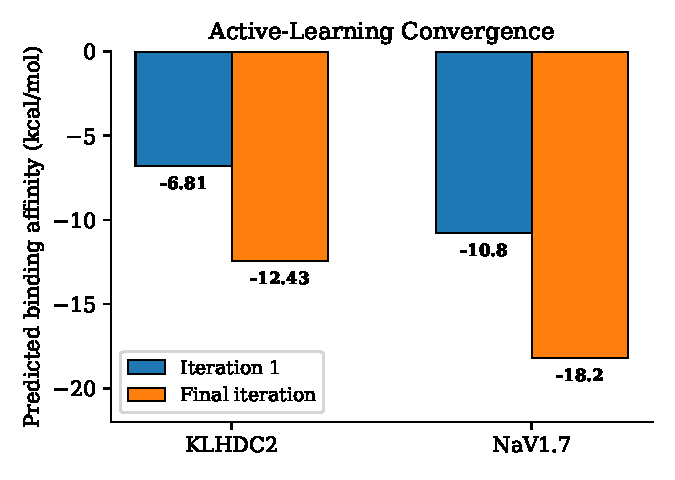
\includegraphics[width=0.6\textwidth]{figures/fig_active_learning.pdf}
\caption{Predicted binding affinity of the top 0.1 percentile compounds
across active-learning iterations for the KLHDC2 and NaV1.7 VSD4 campaigns.
KLHDC2: $-6.81$~kcal/mol (iteration~1) to $-12.43$~kcal/mol (iteration~10).
NaV1.7: $-10.8$~kcal/mol (iteration~1) to $-18.2$~kcal/mol (final iteration).}
\label{fig:active_learning}
\end{figure}

After filtering and clustering the top 1,000 compounds, 54 clustered candidates
were manually examined; 37 were chosen for synthesis and 29 were successfully
synthesized. In the AlphaLISA competition assay, compound~29 (C29) showed the
best activity with IC$_{50} \sim 3$~\textmu M, confirmed by BLI.

% --- KLHDC2 campaign table ---
\begin{table}[htbp]
\centering
\caption{KLHDC2 Enamine REAL virtual screening campaign summary.}
\label{tab:klhdc2_campaign}
\begin{tabular}{ll}
\toprule
Stage & Value \\
\midrule
Library size & $\sim$5.5 billion compounds \\
Synthesis success rate & 80\% \\
Compounds docked & $\sim$6 million (0.11\%) \\
Active-learning iterations & 10 \\
Top 0.1\% affinity, iteration 1 & $-6.81$ kcal/mol \\
Top 0.1\% affinity, iteration 10 & $-12.43$ kcal/mol \\
Re-docked with VSH & 50,000 \\
Filtered and clustered & 54 candidates \\
Selected for synthesis & 37 \\
Successfully synthesized & 29 \\
Best hit (C29) IC$_{50}$ & $\sim$3 \textmu M \\
Focused screen (ZINC22) & $\sim$381,567 hits \\
Focused screen synthesized & 21 \\
Additional hits & 6 (single-digit \textmu M IC$_{50}$) \\
Total KLHDC2 hits & 7 \\
Overall hit rate & 14\% \\
Compute resources & 3000 CPUs + 1 RTX2080 GPU \\
Campaign duration & $<$7 days \\
\bottomrule
\end{tabular}
\end{table}

The KLHDC2--C29 co-crystal structure was determined at 2.0~\AA\ resolution.
The structure reveals that the distal carboxyl group of C29 contacts Arg236,
Arg241, and Ser269; the triazole moiety is nestled among Tyr163, Trp191, and
Trp270 with a stabilizing NH\ldots N hydrogen bond; Lys147 forms a hydrogen
bond with the central carbonyl group; and the tert-butylphenyl group packs
into the auxiliary chamber of the degron-binding pocket. The experimentally
determined binding pose closely matches the computationally predicted pose.

A focused follow-up screen of ZINC22 \citep{tingle2023zinc22} for the
acetyl-amino-methyl-triazole-acetic acid substructure returned approximately
381,567 compounds. Twenty-one were synthesized, and six additional hits showed
single-digit micromolar IC$_{50}$ values, bringing the total to seven
low-micromolar KLHDC2 binders with an overall hit rate of 14\%
(Figure~\ref{fig:hit_rates}).

\subsection{Discovery of Novel NaV1.7 VSD4 Antagonists}

The ZINC22 library \citep{tingle2023zinc22} (approximately 4.1 billion
compounds) was screened against NaV1.7 VSD4 \citep{wang2015nav17methyl} using
the same OpenVS/VSX pipeline. Over 7 active-learning iterations, the predicted
binding affinity of the top 0.1 percentile improved from $-10.8$~kcal/mol
(iteration~1) to $-18.2$~kcal/mol (final iteration)
(Figure~\ref{fig:active_learning}). Approximately 4.5 million compounds
(0.11\%) were docked; the top 100,000 were re-docked with VSH.

% --- NaV1.7 campaign table ---
\begin{table}[htbp]
\centering
\caption{NaV1.7 VSD4 ZINC22 virtual screening campaign summary.}
\label{tab:nav17_campaign}
\begin{tabular}{ll}
\toprule
Stage & Value \\
\midrule
Library size & $\sim$4.1 billion compounds \\
Compounds docked & $\sim$4.5 million (0.11\%) \\
Active-learning iterations & 7 \\
Top 0.1\% affinity, iteration 1 & $-10.8$ kcal/mol \\
Top 0.1\% affinity, final iteration & $-18.2$ kcal/mol \\
Re-docked with VSH & 100,000 \\
Clustered and filtered & 160 examined \\
Selected for synthesis & 10 (Tanimoto $< 0.33$) \\
Successfully synthesized & 9 \\
Hits (IC$_{50} < 10$ \textmu M) & 4 \\
Hit rate & 44.4\% \\
Compute resources & 3000 CPUs + 1 RTX2080 GPU \\
Campaign duration & $<$7 days \\
\bottomrule
\end{tabular}
\end{table}

After clustering, filtering, and manual inspection, 10 structurally novel
molecules (Tanimoto similarity $< 0.33$ to known ChEMBL NaV1.7 inhibitors)
were selected and 9 were synthesized. Whole-cell patch-clamp electrophysiology
on hNaV1.7 in HEK-293 cells identified four compounds with IC$_{50} < 10$
\textmu M, yielding a 44.4\% hit rate (Figure~\ref{fig:hit_rates}).

% --- Hit rates figure ---
\begin{figure}[htbp]
\centering
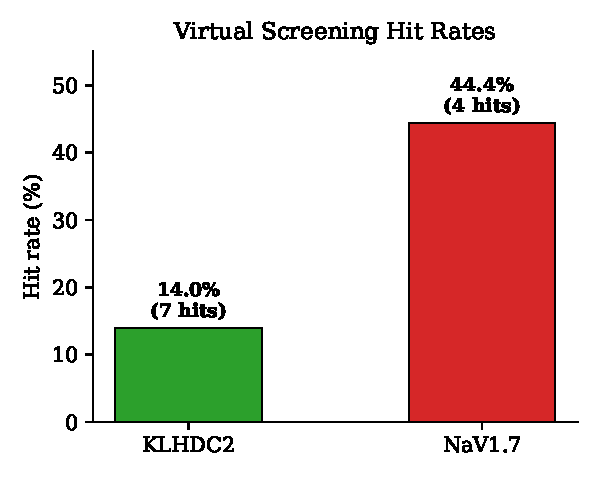
\includegraphics[width=0.55\textwidth]{figures/fig_hit_rates.pdf}
\caption{Experimental hit rates for the KLHDC2 and NaV1.7 VSD4 virtual
screening campaigns. KLHDC2: 7 hits (14\% hit rate); NaV1.7: 4 hits with
IC$_{50} < 10$~\textmu M (44.4\% hit rate).}
\label{fig:hit_rates}
\end{figure}

The best compound, Z8739902234, exhibited inactivated-state IC$_{50}$ =
1.32~\textmu M (95\% CI: 1.14--1.55) and resting-state IC$_{50}$ =
13.1~\textmu M (95\% CI: 12.78--13.45), demonstrating state-dependent
inhibition (Figure~\ref{fig:nav17_ic50}). Z8739902234 showed moderate
selectivity: NaV1.7 IC$_{50}$ = 1.33~\textmu M (95\% CI: 1.14--1.55),
NaV1.5 IC$_{50}$ = 5.14~\textmu M (95\% CI: 4.74--5.55), hERG IC$_{50}$ =
6.27~\textmu M (95\% CI: 5.27--7.37). The second-best compound, Z8739905023,
had an inactivated-state IC$_{50}$ = 2.23~\textmu M (95\% CI: 2.14--2.46).

% --- NaV1.7 IC50 figure ---
\begin{figure}[htbp]
\centering
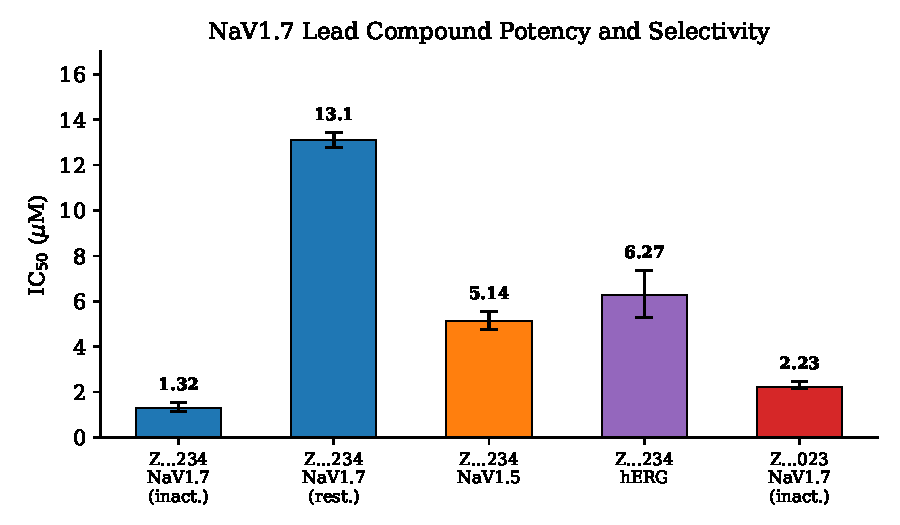
\includegraphics[width=0.7\textwidth]{figures/fig_nav17_ic50.pdf}
\caption{IC$_{50}$ values (mean, 95\% CI) for the two best NaV1.7 VSD4 lead
compounds. Z8739902234: inactivated-state IC$_{50}$ = 1.32~\textmu M
(1.14--1.55), resting-state IC$_{50}$ = 13.1~\textmu M (12.78--13.45);
selectivity against NaV1.5 (5.14~\textmu M, 4.74--5.55) and hERG
(6.27~\textmu M, 5.27--7.37). Z8739905023: inactivated-state IC$_{50}$ =
2.23~\textmu M (2.14--2.46).}
\label{fig:nav17_ic50}
\end{figure}

% --- NaV1.7 IC50 table ---
\begin{table}[htbp]
\centering
\caption{Concentration--response and selectivity data for lead NaV1.7 VSD4
compounds. IC$_{50}$ values in \textmu M (mean, 95\% CI) from whole-cell
patch-clamp electrophysiology.}
\label{tab:nav17_ic50}
\begin{tabular}{llcc}
\toprule
Compound & Channel / State & IC$_{50}$ (\textmu M) & 95\% CI \\
\midrule
Z8739902234 & hNaV1.7, inactivated & 1.32 & 1.14--1.55 \\
Z8739902234 & hNaV1.7, resting & 13.1 & 12.78--13.45 \\
Z8739902234 & hNaV1.5 & 5.14 & 4.74--5.55 \\
Z8739902234 & hERG & 6.27 & 5.27--7.37 \\
Z8739905023 & hNaV1.7, inactivated & 2.23 & 2.14--2.46 \\
\bottomrule
\end{tabular}
\end{table}


% ============================================================
% DISCUSSION
% ============================================================
\section{Discussion}

The results presented here establish RosettaGenFF-VS and RosettaVS as leading
physics-based methods for ligand docking and virtual screening. The combination
of high docking accuracy and efficient conformational sampling enables the
virtual screening protocol to locate the correct binding minimum of
protein-ligand complexes more effectively than competing approaches. Unlike
many existing methods that perform well primarily on hydrophobic, deep, and
large pockets, RosettaGenFF-VS demonstrates strong performance on more polar,
shallower, and smaller pockets, likely due to a better balance of
protein-ligand versus intra-ligand molecular energies achieved by the revised
force field.

The two parallel drug-discovery campaigns illustrate the practical utility of
the platform. Both the KLHDC2 screen (approximately 5.5 billion Enamine REAL
compounds) and the NaV1.7 VSD4 screen (approximately 4.1 billion ZINC22
compounds) completed in under seven days on a local HPC cluster with 3000 CPUs
and a single RTX2080 GPU, with only approximately 0.11\% of each library
explicitly docked. The KLHDC2 campaign produced seven low-micromolar binders
(14\% hit rate), the best of which (C29, IC$_{50} \sim 3$~\textmu M) was
validated by a 2.0~\AA\ X-ray co-crystal structure showing close agreement
with the predicted binding pose. The NaV1.7 campaign yielded four hits with
IC$_{50} < 10$~\textmu M (44.4\% hit rate), with the best compound
(Z8739902234) displaying state-dependent inhibition (inactivated-state
IC$_{50}$ = 1.32~\textmu M) and moderate selectivity over NaV1.5 and hERG.

Several avenues for future improvement are anticipated. GPU acceleration of
Rosetta docking would further reduce wall-clock time. Generative AI approaches
for efficient pose generation could complement the current sampling strategy,
particularly as advances in protein structure prediction
\citep{tunyasuvunakool2021alphafold} continue to expand the set of
structurally characterized targets amenable to virtual screening
\citep{irwin2005metalloenzyme}. Refinement of the active-learning surrogate
models would improve chemical-space exploration, and incorporation of a
generalizable deep-learning-based score function could further enhance
discrimination of true binders. Template-guided
screening using known non-small-molecule binders such as macrocycles or antibody
loops as structural templates represents another promising extension. These
developments, combined with the open-source nature of the platform, position
OpenVS as a foundation for continued advances in structure-based virtual
screening at the multi-billion compound scale.


% ============================================================
% BIBLIOGRAPHY
% ============================================================
\bibliographystyle{plainnat}
\bibliography{references}

\end{document}
